\documentclass[letter]{article}
\usepackage{enumerate}
\usepackage{amsmath}
\usepackage{amssymb}
\usepackage{amsfonts}
\usepackage{amsthm}
\usepackage{latexsym}
\usepackage{mathrsfs}
\usepackage{eufrak}
\usepackage[pdftex]{graphicx}
\usepackage{color}
\usepackage{mathrsfs}
\setlength{\topmargin}{-0.5in} \setlength{\textwidth}{6.5in}
\setlength{\oddsidemargin}{0.0in} \setlength{\textheight}{9.1in}
\usepackage[table]{xcolor}
\graphicspath{{./cse373hw1/}}

\newlength{\pagewidth}
\setlength{\pagewidth}{6.5in} \pagestyle{empty}

\newcommand{\R}{\mathbb{R}}
\newcommand{\N}{\mathbb{N}}
\newcommand{\B}{\mathfrak{B}}
\newcommand{\Z}{\mathbb{Z}}
\newtheorem{theorem}{Theorem}[section]
\newtheorem{lemma}[theorem]{Lemma}
\newtheorem{proposition}[theorem]{Proposition}
\newtheorem{corollary}[theorem]{Corollary}

\newenvironment{definition}[1][Definition]{\begin{trivlist}
\item[\hskip \labelsep {\bfseries #1}]}{\end{trivlist}}
\newenvironment{example}[1][Example]{\begin{trivlist}
\item[\hskip \labelsep {\bfseries #1}]}{\end{trivlist}}
\newenvironment{remark}[1][Remark]{\begin{trivlist}
\item[\hskip \labelsep {\bfseries #1}]}{\end{trivlist}}

\title{CSE 373 Spring 2010 HW \#1}
\date{}
\author{Chao Xu(106978083), Xiaodi Zheng(106718764)}
\begin{document}
\maketitle
\vspace{-.5in}
\section{}
All graphs are data size vs milliseconds.
2-to-n.c\\
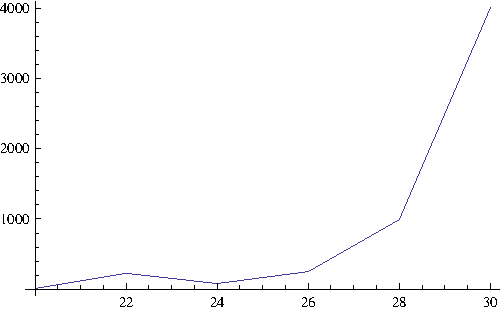
\includegraphics[scale=1]{2-to-n.pdf}

binary-search.c\\
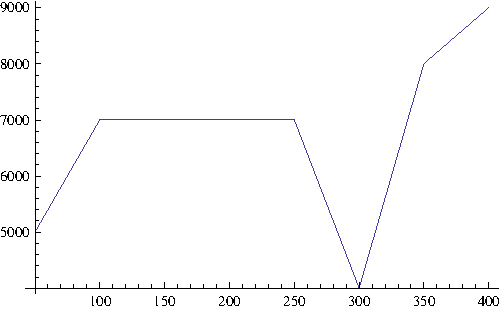
\includegraphics[scale=1]{binarysearch.pdf}

fac_time.c\\
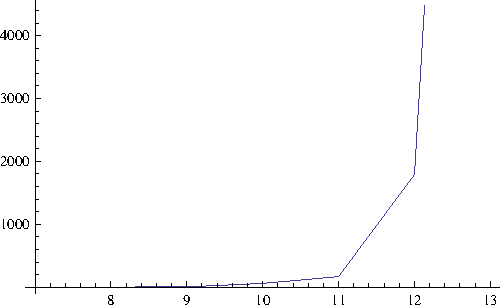
\includegraphics[scale=1]{fact.pdf}

insert-sort.c\\
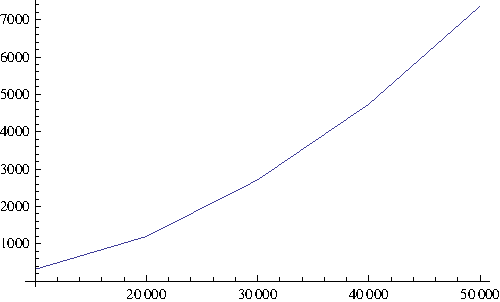
\includegraphics[scale=1]{insert.pdf}

merge-sort.c\\
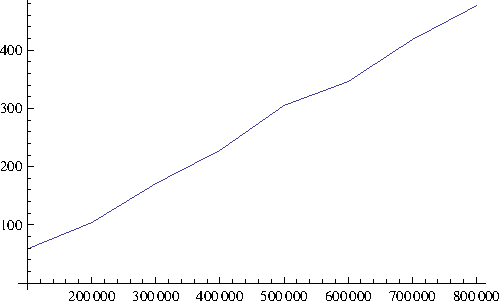
\includegraphics[scale=1]{mergesort.pdf}

seq-search.c\\
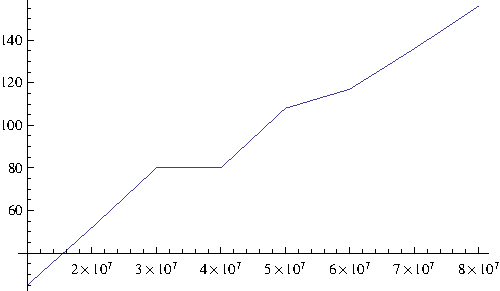
\includegraphics[scale=1]{seqsort.pdf}

triple.c\\
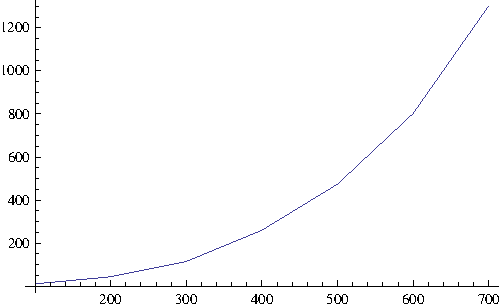
\includegraphics[scale=1]{triple,pdf.pdf}

Programs do behave roughly as expected by theory.

\newpage
\section{}
\subsection*{1-17}
Let $P(n)$ be the predicate ``A tree with $n$ vertices has exactly $n-1$ edges''.\\
\emph{base case:} $P(1)$ is true. A tree with $1$ vertex has no edges.\\
\emph{inductive step:} Suppose $P(n)$ is true. Prove $P(n+1)$ is true.\\
Let $T$ be a tree with $n+1$ vertices. Remove a leaf from the tree. The leaf has only one edge. We have a tree $T'$ with one less edge than $T$. $T'$ is a tree with $n$ vertices. By $P(n)$. $T'$ has $n-1$ edges. $T$ has $n$ edges. Proves $P(n+1)$ is true.

\subsection*{1-19}
\paragraph*{(a)}
No. Even if each book I own has 1000 pages, I need 1000 books to have 1 million pages.
\paragraph*{(b)}
Each stack of book have around 10000 pages. Each bookshelf have 6 stacks. There are around 500 bookshelfs in the library. There are around 10000*6*500 = 30 million pages in the library.

\newpage
\section{}
\subsection*{2-7}
\paragraph*{(a)}
True. $2^{n+1} = 2\times 2^n = O(2^n)$.
\paragraph*{(b)}
False. $2^{2n} = 2^n\times 2^n \neq c\times 2^n$ where $c$ is a constant.

\subsection*{2-8}
\paragraph*{(a)}
$f(n) = \log n^2 = 2 \log n = \Theta (\log n)$\\
$g(n) = \log n + 5= \Theta(\log n)$\\
$f(n) = \Theta(g(n))$

\paragraph*{(b)}
$f(n) = \sqrt{n} = \Theta(n^\frac{1}{2})$\\
$g(n) = \log n^2 = 2 \log n = \Theta(\log n)$\\
$f(n) = \Omega(g(n))$\\

\paragraph*{(c)}
$f(n) = \Theta((\log n)^2)$\\
$g(n) = \Theta(\log n)$\\
$f(n) = \Omega(g(n))$

\paragraph*{(d)}
$f(n) = \Theta(n)$\\
$g(n) = \Theta((\log n)^2)$\\
$f(n) = \Omega(g(n))$

\paragraph*{(e)}
$f(n) = n \log n + n \Theta(n\log n)$\\
$g(n) = \Theta(\log n)$\\
$f(n) = \Omega(g(n))$

\paragraph*{(f)}
$f(n) = 10 = \Theta(1)$\\
$g(n) = \log 10 = \Theta(1)$\\
$f(n) = \Theta(g(n))$

\paragraph*{(g)}
$f(n) = \Theta(2^n)$\\
$g(n) = \Theta(n^2)$\\
$f(n) = \Omega(g(n))$

\paragraph*{(h)}
$f(n) = \Theta(2^n)$\\
$g(n) = \Theta(3^n)$\\
$cf(n)<g(n)$ for all $c$ for sufficiently large $n$.\\
$f(n) = O(g(n))$
\newpage

\section{}
\subsection*{2-19}
Ones in the same curly brackets are in the same order\\
$(\frac{1}{3})^n$,
$6$,
$\log \log n$,
$\{\ln n,\log n\}$,
$(\log n)^2$,
$\frac{n}{\log n}$,
$n^{\frac{1}{3}} + \log n$,
$\sqrt{n}$,
$n$,
$n\log n$,
$\{n^2,n^2 + \log n\}$,
$n^3$,
$n^5$,
$(\frac{3}{2})^n$,
$2^n$,
$n!$

\newpage
\section{}
\subsection*{2-21}
\begin{enumerate}[(a)]
 \item true
 \item false
 \item true
 \item false
 \item true
 \item true
 \item false
\end{enumerate}

\subsection*{2-22}
\begin{enumerate}[(a)]
 \item $f(n) = \Omega(g(n))$
 \item $f(n) = O(g(n))$
 \item $f(n) = \Omega(g(n))$
\end{enumerate}

\subsection*{2-23}
\begin{enumerate}[(a)]
 \item Yes, insertion sort is an example.
 \item Yes, $cn = O(n^2)$
 \item Yes, insertion sort
 \item No, For some input it has to have $\Omega(n^2)$
 \item yes $100n^2 = \Theta(n^2)$, $20n^2 - n\log_2 n = \Theta(n^2)$. $f(n) = \Theta(n^2)$
\end{enumerate}

\subsection*{2-24}
\begin{enumerate}[(a)]
 \item False, $(\frac{3}{2})^n 2^n \neq c 2^n$
 \item True. $\log 3^n = n \log 3= \Theta(n)$, $\log 2^n = n \log 2 = \Theta(n)$.
 \item True, refer to part (a).
 \item True, refer to part (b).
\end{enumerate}

\newpage
\section{}
\subsection*{3-2}
\begin{verbatim}
 reverse(L){
  tmp = find_last_element(L);
  reverse_helper(L);
  return tmp;
 }

 reverse_helper(L){
  if(L != nil && L.next !=nill){
   reverse_helper(L.next);
    L.next.next = L;
    L.next = nil;
  }
  return L;
 }
\end{verbatim} 

\newpage
\section{}
\subsection*{3-4}
An array $A$ of size $n$.
\begin{enumerate}
 \item insert(int $i$): Set $A[i]$ to $1$. $O(1)$
 \item delete(int $i$): Set $A[i]$ to $0$. $O(1)$
 \item search(int $i$): return $A[i]$==1. $O(1)$
\end{enumerate}

\newpage
\section{}
\subsection*{3-10}

Let $B$ be a binary search tree that store the extra room of all bins. For a ball with weight $i$, search $B$ for the smallest number larger than $i$. Add $i$ into that bin, and update the binary tree. If no such number exists, create a new bin and put $i$ in it. Then insert the new bin into $B$.

Find the smallest number larger than or equal to $i$ in a binary search tree is $O(\log n)$ operation, where $n$ is the amount of nodes in the tree. The algorithm tries to find $i$. If a pointer is on node $k$ and found $i$ doesn't exist. Then the number larger than $i$ must be $k.right$ or $k.parent.right$ or $k.parent.parent.right$ and so on. There is at most $O(\log n)$ numbers to check.

For the worst-fit heuristic. Let $P$ be a priority queue of bins that is ordered by the size of extra space. Put the ball in the bin that's on the top of the priority queue if it fits in the bin, then update the priority queue. If no bin in the priority queue can hold the ball, create a new bin and put the ball in it.

\newpage
\section{}
\subsection*{3-11}
\begin{enumerate}[(a)]
 \item Matrix $A[i][j]$ holds the smallest value in $x_i,\ldots,x_j$.
 \item Suppose $n = 2^m$ for some integer $m$ for convenience. For all $0 \leq k\leq \log_2 n$ and all $0 \leq m \leq \frac{n}{2^k}$, precompute the smallest value between $x_{m \frac{n}{2^k}+1 }$ and $x_{(m+1)\frac{n}{2^k} }$. Let's call the partition $x_{m \frac{n}{2^k}+1}$ and $x_{(m+1)\frac{n}{2^k}}$ the $m$-th-$2^k$-partition.\\
For any $i,j$, there exist $O(\log n)$ partitions that combined together contains all integers in $x_i,\ldots,x_j$.

Pseudocode. Suppose $n = 2^k$ for some $k$.\\
Suppose the min\_interval(m,k) function returns the smallest value in the $m$-th-$2^k$-partition of x. It's precomputed, thus it's $O(1)$ algorithm.
\begin{verbatim}
 minimum(int i, int j, int[] x[n]){
   if(i==j){
     return x[i];
   }
   int k = floor(log_2(j-i));
   int m = ceil(i/(n/(2^k)));
   return min(minimum(i,m*n/2^k,x),min_interval(m,k),minimum((m+1)*n/2^k,j,x));
 }
\end{verbatim} 
$i,j = 4,16 $


\begin{tabular*}{1\textwidth}{@{\extracolsep{\fill}} |c|l|l|l|l|l|l|l|l|l|l|l|l|l|l|l|l|}
  \hline
& 1 & 3 & 5 & \cellcolor[gray]{0.9}7 & \cellcolor[gray]{0.9}2 & \cellcolor[gray]{0.9}4 & \cellcolor[gray]{0.9}6 & \cellcolor[gray]{0.9}8 & \cellcolor[gray]{0.9}9 & \cellcolor[gray]{0.9}10 & \cellcolor[gray]{0.9}11 & \cellcolor[gray]{0.9}12 & \cellcolor[gray]{0.9}13 & \cellcolor[gray]{0.9}14 & \cellcolor[gray]{0.9}15 & \cellcolor[gray]{0.9}16\\
  \hline
\end{tabular*}

\begin{tabular*}{1\textwidth}{@{\extracolsep{\fill}}|c|l|l|}
  \hline
& 1 & \cellcolor[gray]{0.9} 9\\
  \hline
\end{tabular*}

\begin{tabular*}{1\textwidth}{@{\extracolsep{\fill}} |c|l|l|l|l|}
  \hline
& 1 & \cellcolor[gray]{0.9}2 & 9 & 13\\
  \hline
\end{tabular*}

\begin{tabular*}{1\textwidth}{@{\extracolsep{\fill}} |c|l|l|l|l|l|l|l|l|}
  \hline
& 1 & 5 & 2 & 6 & 9 & 11 & 13 & 15\\
  \hline
\end{tabular*}

\begin{tabular*}{1\textwidth}{@{\extracolsep{\fill}} |c|l|l|l|l|l|l|l|l|l|l|l|l|l|l|l|l|}
  \hline
& 1 & 3 & 5 & \cellcolor[gray]{0.9}7 & 2 & 4 & 6 & 8 & 9 & 10 & 11 & 12 & 13 & 14 & 15 & 16\\
  \hline
\end{tabular*}

Returns smallest of $9, 2$ and $7$. Which is two.

\end{enumerate}

\end{document}
\theend
